\subsection{Implementation}

Main technologies used for creating web application are: NodeJS, Express, HandlebarsJS and Mongoose. Here is the role of each tool:
\begin{itemize}
  \item NodeJS
  \begin{itemize}
    \item Backbone of the project - backend
  \end{itemize}
  \item Express
  \begin{itemize}
    \item Routing across web pages
  \end{itemize}
  \item HandlebarsJS
  \begin{itemize}
    \item Rendering HTML with data inside
  \end{itemize}
  \item Mongoose
  \begin{itemize}
    \item Getting the data from MongoDB cluster.
  \end{itemize}
\end{itemize}

Homepage, consisting of main actions:
\begin{itemize}
  \item login,
  \item forgotten password,
  \item registration.
\end{itemize}
\begin{figure}[H]
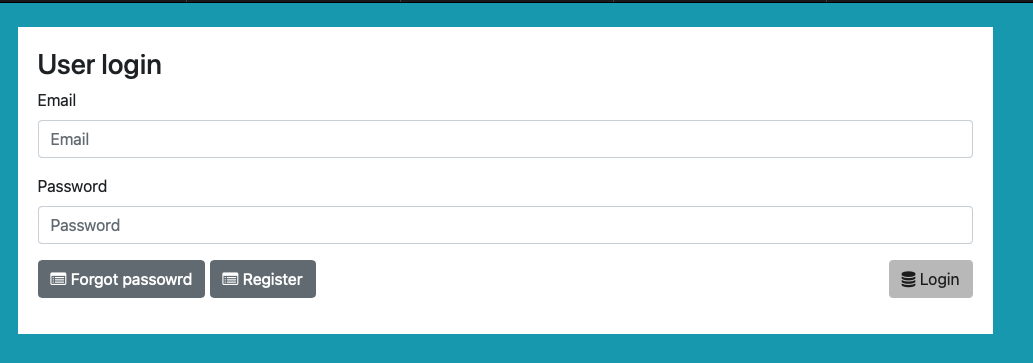
\includegraphics[scale=0.4]{img/homePage.jpeg}
\centering
\caption{Home page}
\end{figure}

If user has forgotten the password, they would need to fill in the section with full name (name and surname ) and email. To send emails, we can integrate sendgrid API. With that, automatic emails will be send for password reset. Unfortunately this is not implemented yet (email sending). 
\begin{figure}[H]
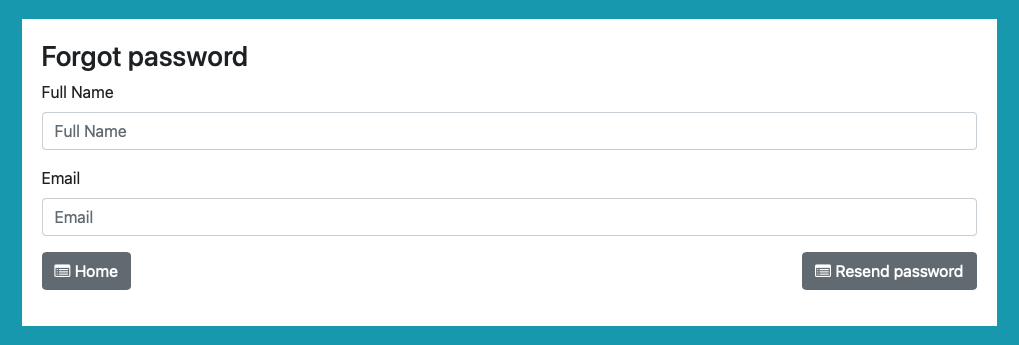
\includegraphics[scale=0.4]{img/forgotPassowrd.jpeg}
\centering
\caption{Forgotten password}
\end{figure}

User needs to fill in the form to register. Once done, he/she is saved to MongoDB and they are redirected to homepage.
\begin{figure}[H]
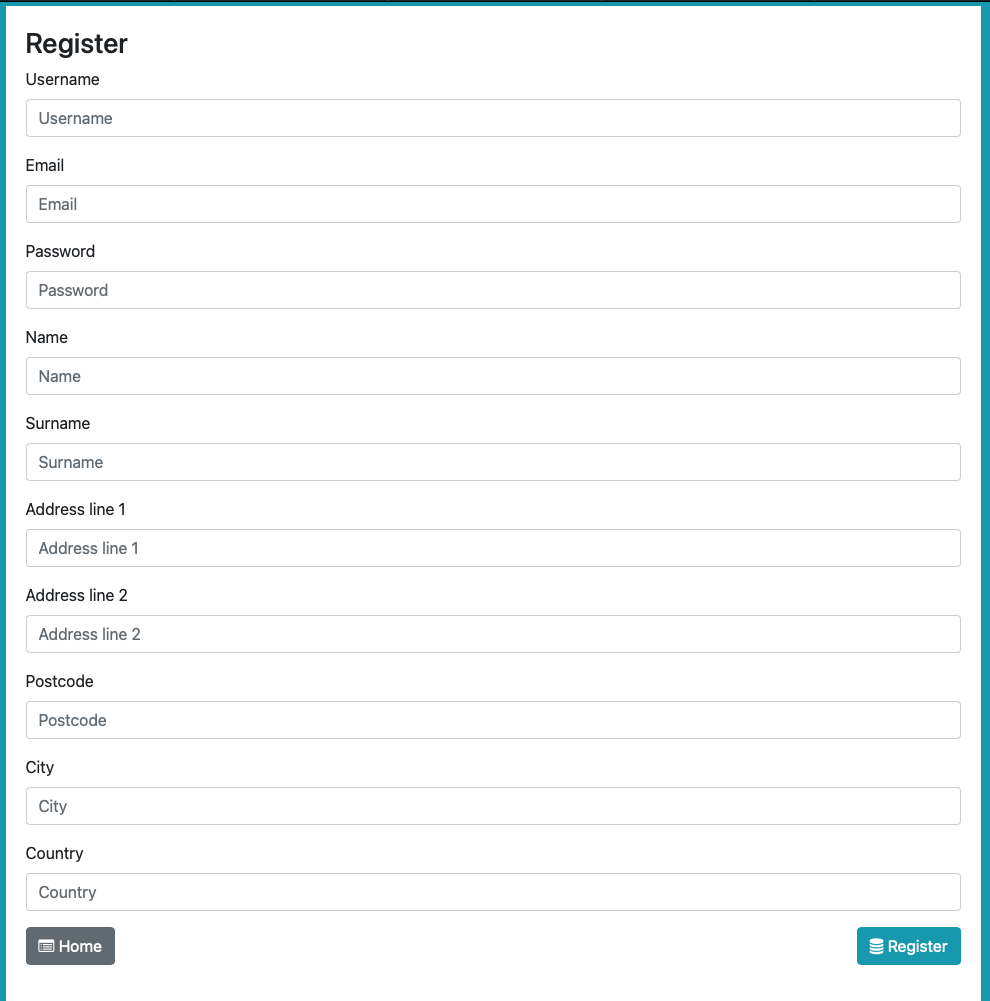
\includegraphics[scale=0.4]{img/register.jpeg}
\centering
\caption{Register section}
\end{figure}

Once user is logged in, classes of devices are shown. This is list of supported classes (under device type) and number of devices user has registered. If new device type comes to support, user would have number of devices as 0 and could add new device by selecting pencil (see all).
\begin{figure}[H]
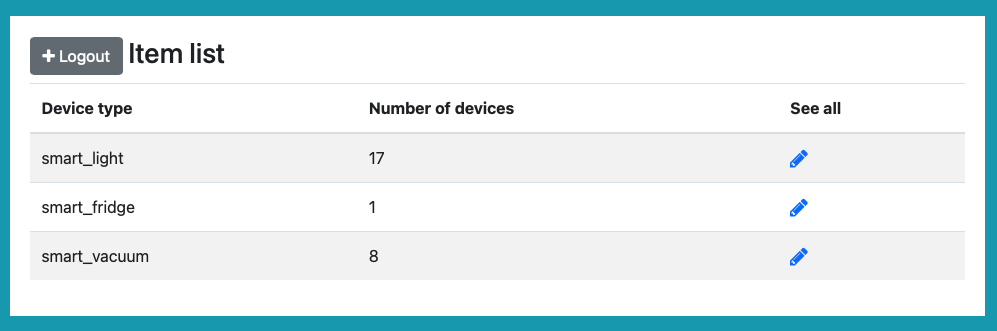
\includegraphics[scale=0.4]{img/deviceClasses.jpeg}
\centering
\caption{Devices classified}
\end{figure}

Upon selecting device type, all of the devices from that sections are displayed. User can also see some of the settings on top. There are also options to add, delete and update the device.
\begin{figure}[H]
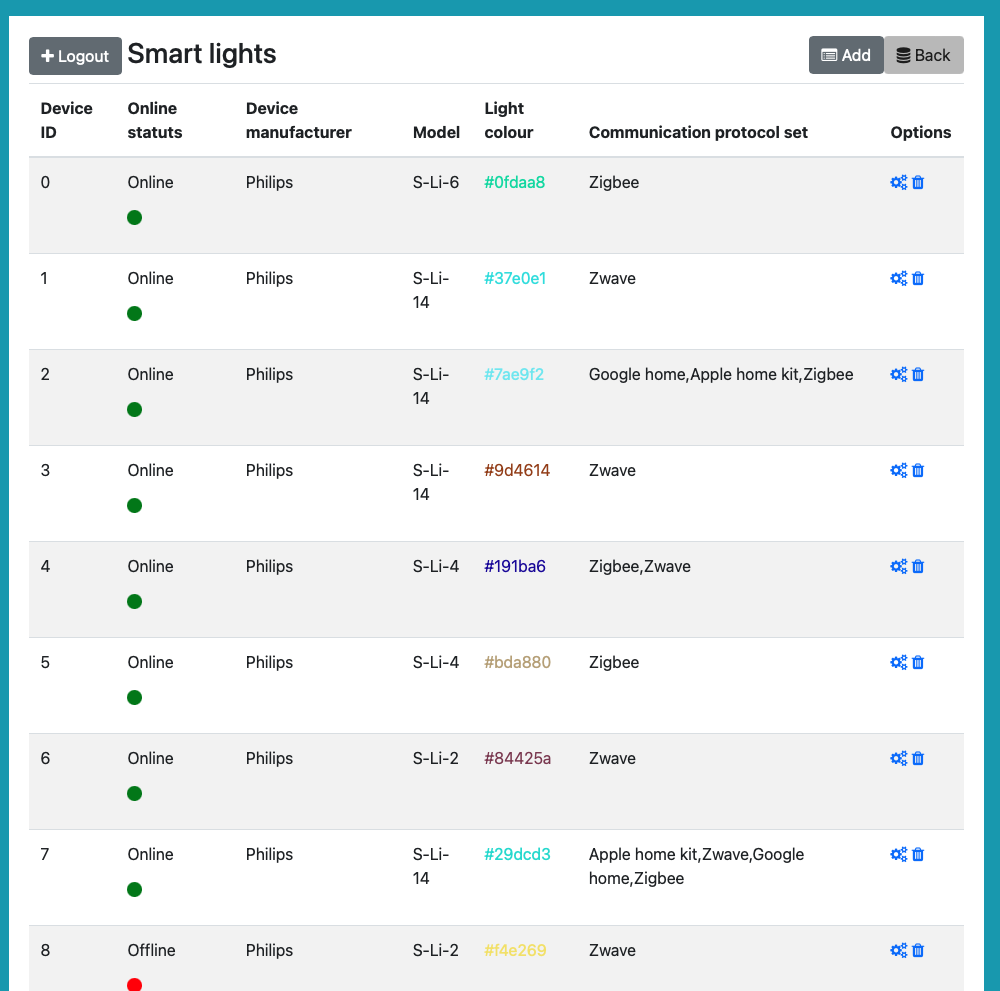
\includegraphics[scale=0.4]{img/listOfDevices.jpeg}
\centering
\caption{List of devices}
\end{figure}

Adding new device is simple. User needs to select information that is supported and correct for him/her. For example, on drop down menu, user selects manufacturer and then model from that manufacturer.
\begin{figure}[H]
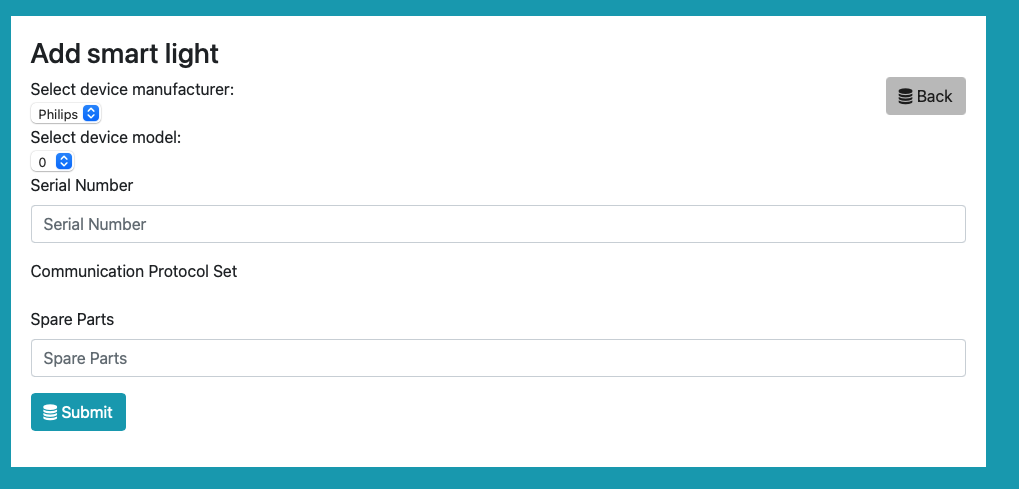
\includegraphics[scale=0.4]{img/addDevice.jpeg}
\centering
\caption{Add device}
\end{figure}

If user wants to remove the device, they can select bin icon and they will see a popup to confirm if they want to remove device or not.
\begin{figure}[H]
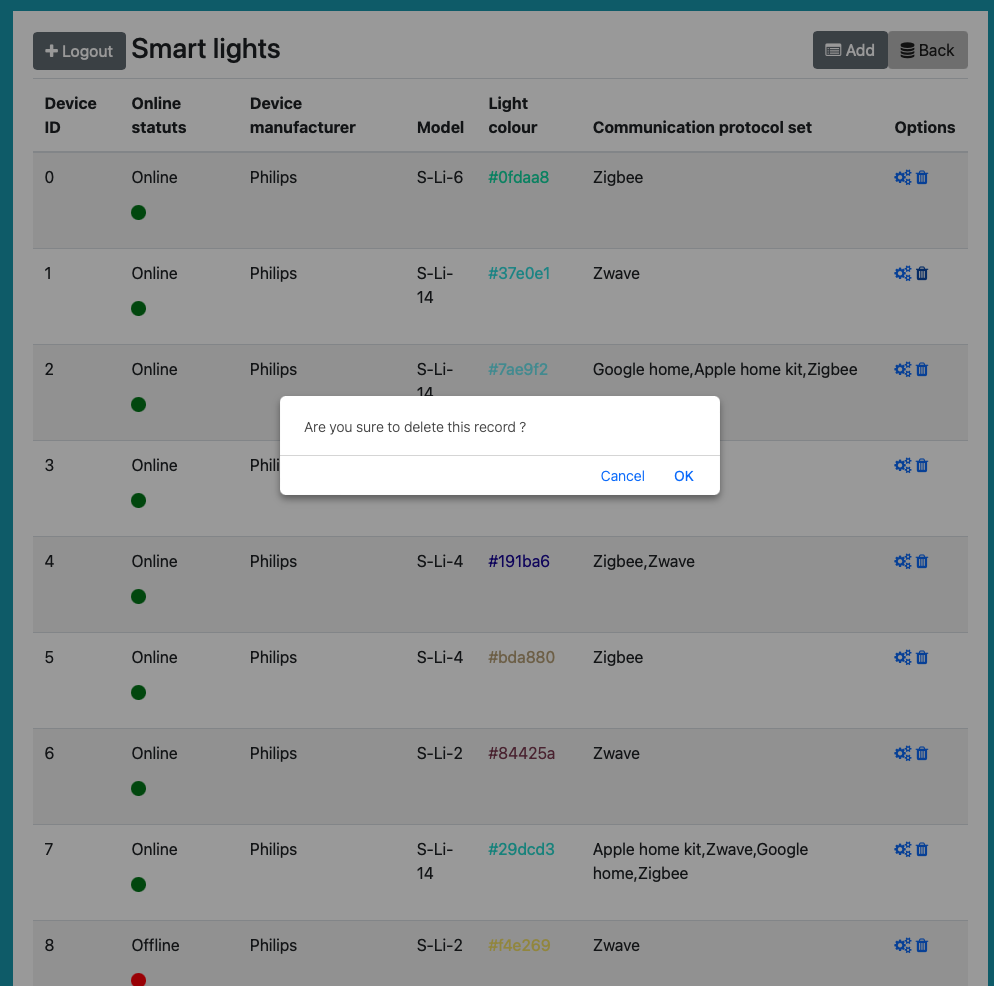
\includegraphics[scale=0.4]{img/removeDevice.jpeg}
\centering
\caption{Remove device}
\end{figure}

Update section reads device information and displays it on web page. User can then edit section they desire.
\begin{figure}[H]
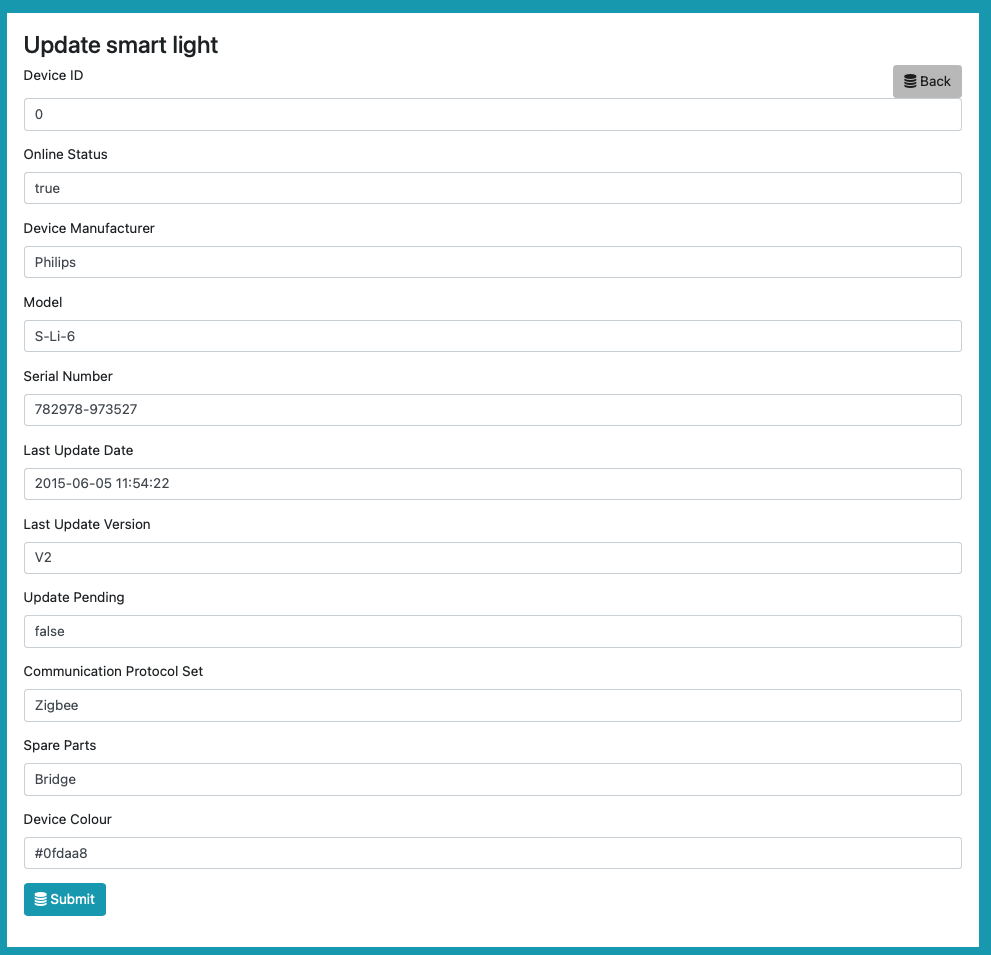
\includegraphics[scale=0.4]{img/editDevice.jpeg}
\centering
\caption{Edit device}
\end{figure}